\newpage
\section{Lösungskonzept}
\subsection[Designkonzept]{Designkonzept}
Das Design des Admin-UIs wurde von einem seperaten Designerteam erstellt, welches nah mit dem Kunden zusammengearbeitet hat.

Die Mockups orientieren sich an den Anforderungen \hyperref[Tab:A4]{A4}, \hyperref[Tab:A5]{A5}, \hyperref[Tab:A6]{A6} und \hyperref[Tab:A7]{A7}. Sie fügen jedoch noch andere Elemente hinzu, um für ein gutes \gls{ux} zu sorgen. Dazu gehören:
\begin{itemize}
    \item Die Unterteilung der Eingabefelder mit der dazu passenden Überschrift.
    \item Platzhalter in den Eingabefeldern, um besser zu erkennen, was in die Felder eingetragen werden muss.
\end{itemize}

Anhand der Kundenanforderungen und den \gls{ux}-Anforderungen hat wurden von dem Designteam einige Mockups für das Admin-UI erstellt, welche dem Entwicklerteam als Leitbild dienen soll. \\\\
\textit{Notiz: Um die Anonymität des Kunden zu wahren, wurden einige Stellen der Mockups geschwärzt.}

\subsubsection[short]{Mockups für das Admin-UIs}
\begin{figure}[H]
    \centering
    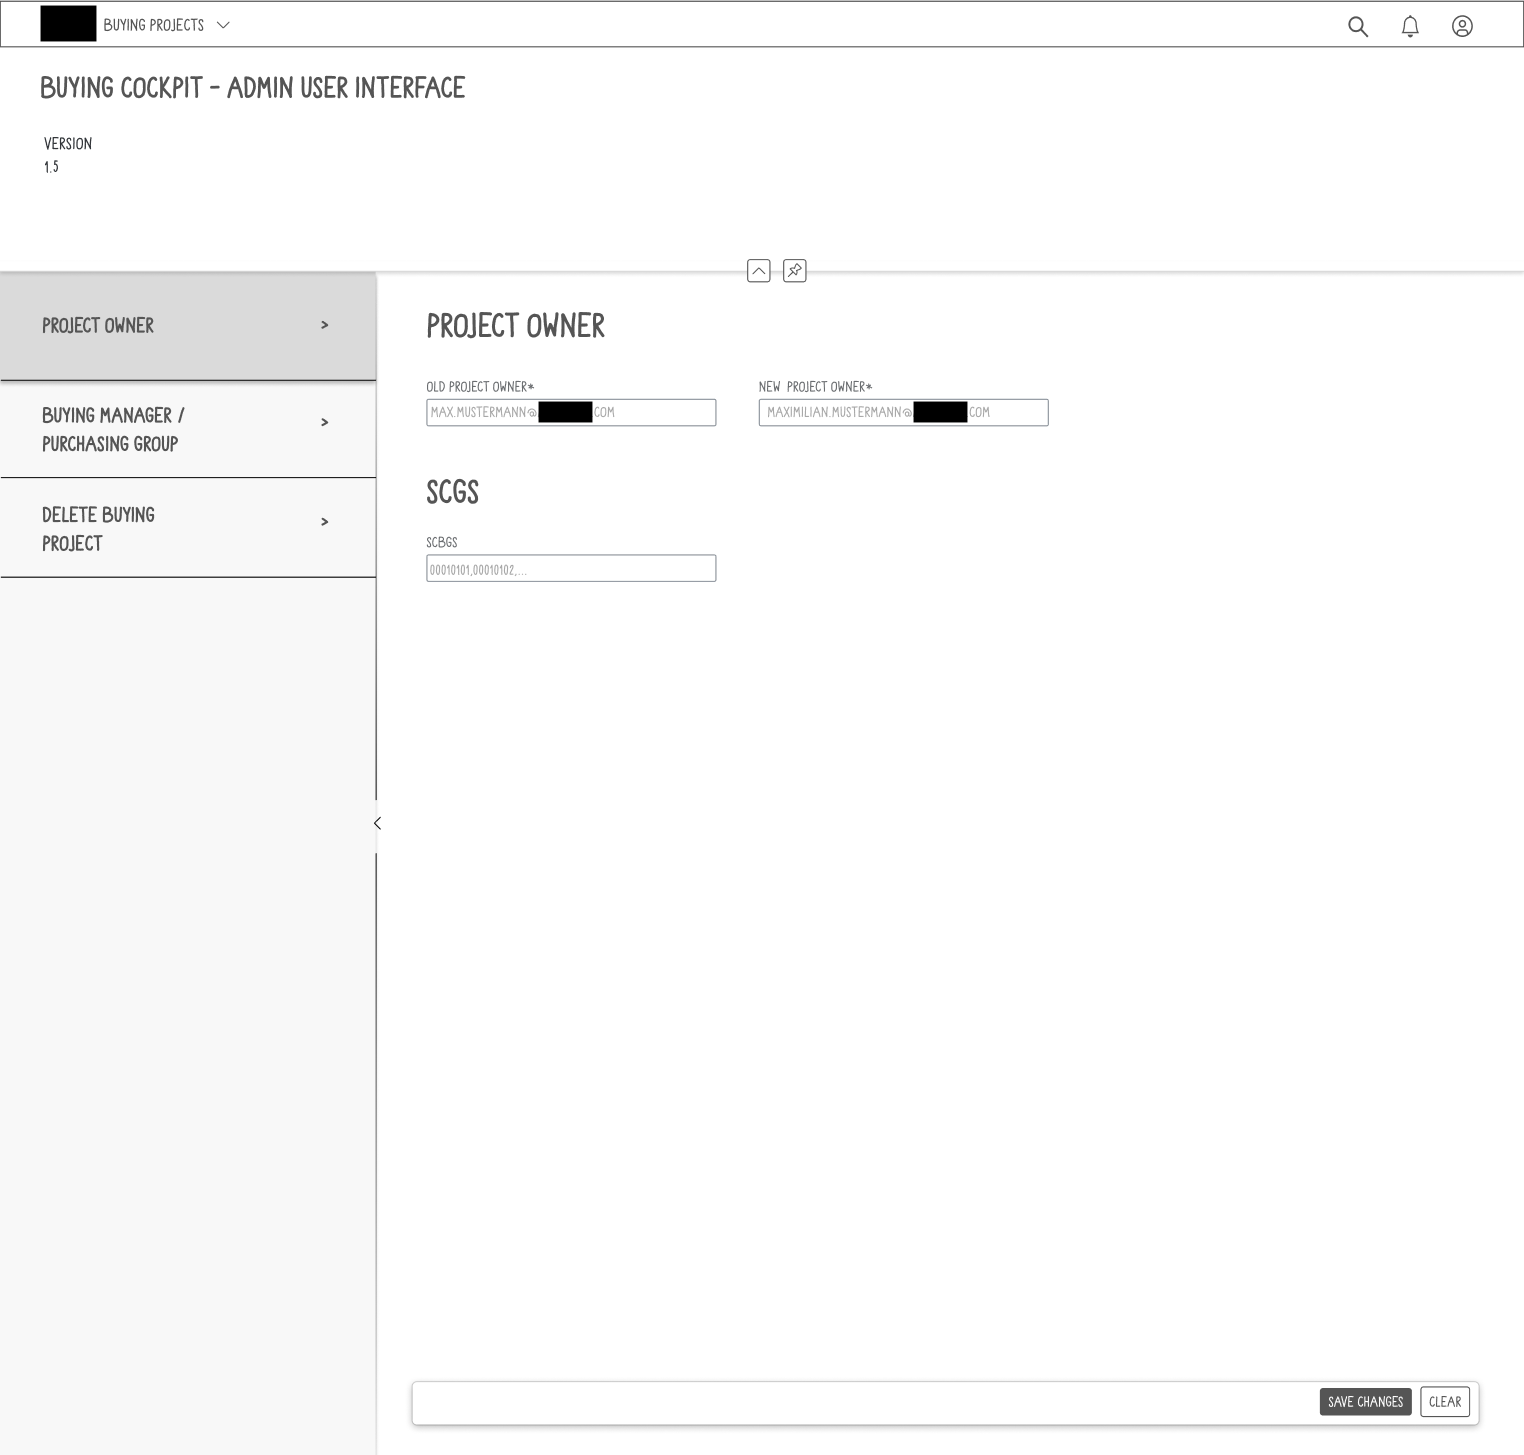
\includegraphics[width=\linewidth]{Images/Mockup_PO_anonym.png}
    \caption[Mockup: Admin-UI Projekowner Seite]{Mockup: Admin-UI Projekowner Seite}
\end{figure}

\begin{figure}[H]
    \centering
    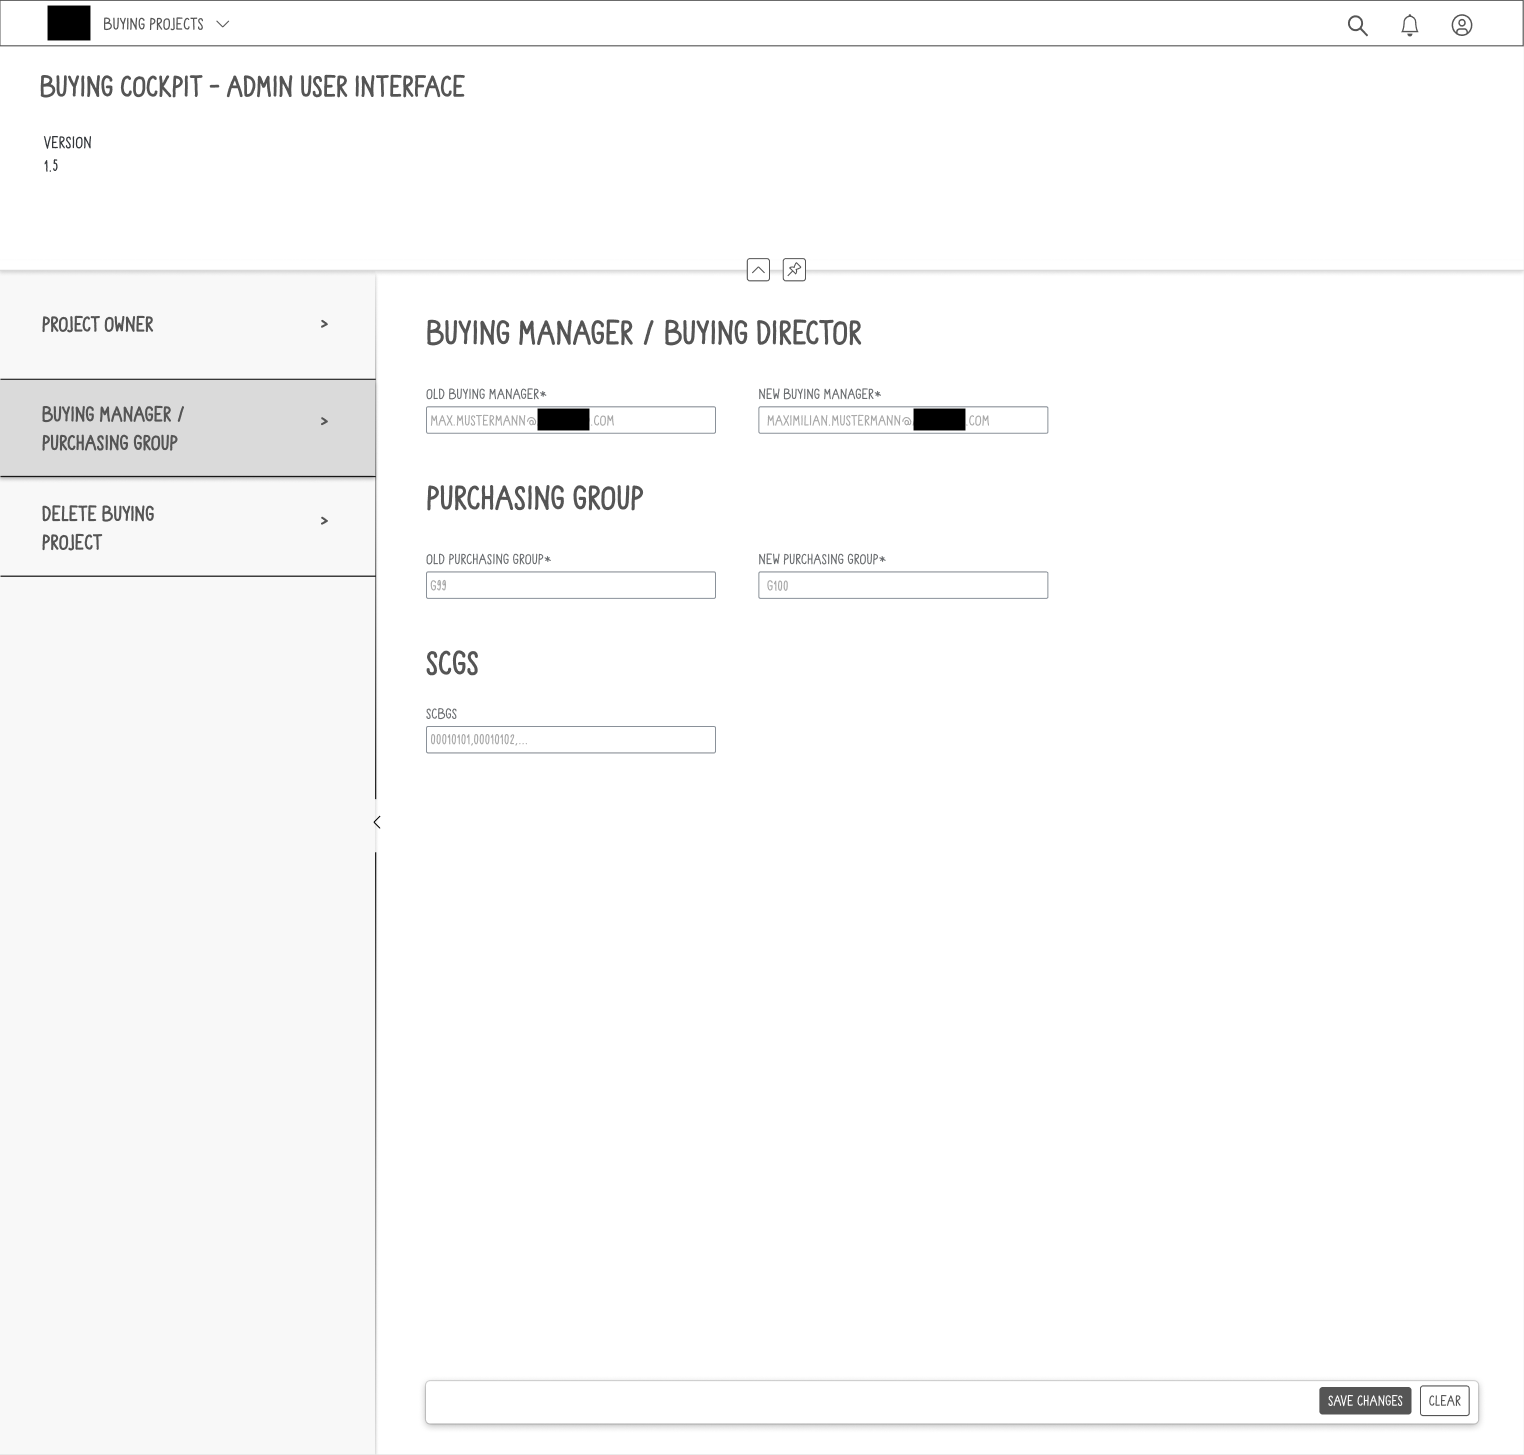
\includegraphics[width=\linewidth]{Images/Mockup_PM_anonym.png}
    \caption[Mockup: Admin-UI Projektmanager und Käufergruppe Seite]{Mockup: Admin-UI Projektmanager und Käufergruppe Seite}
\end{figure}

\begin{figure}[H]
    \centering
    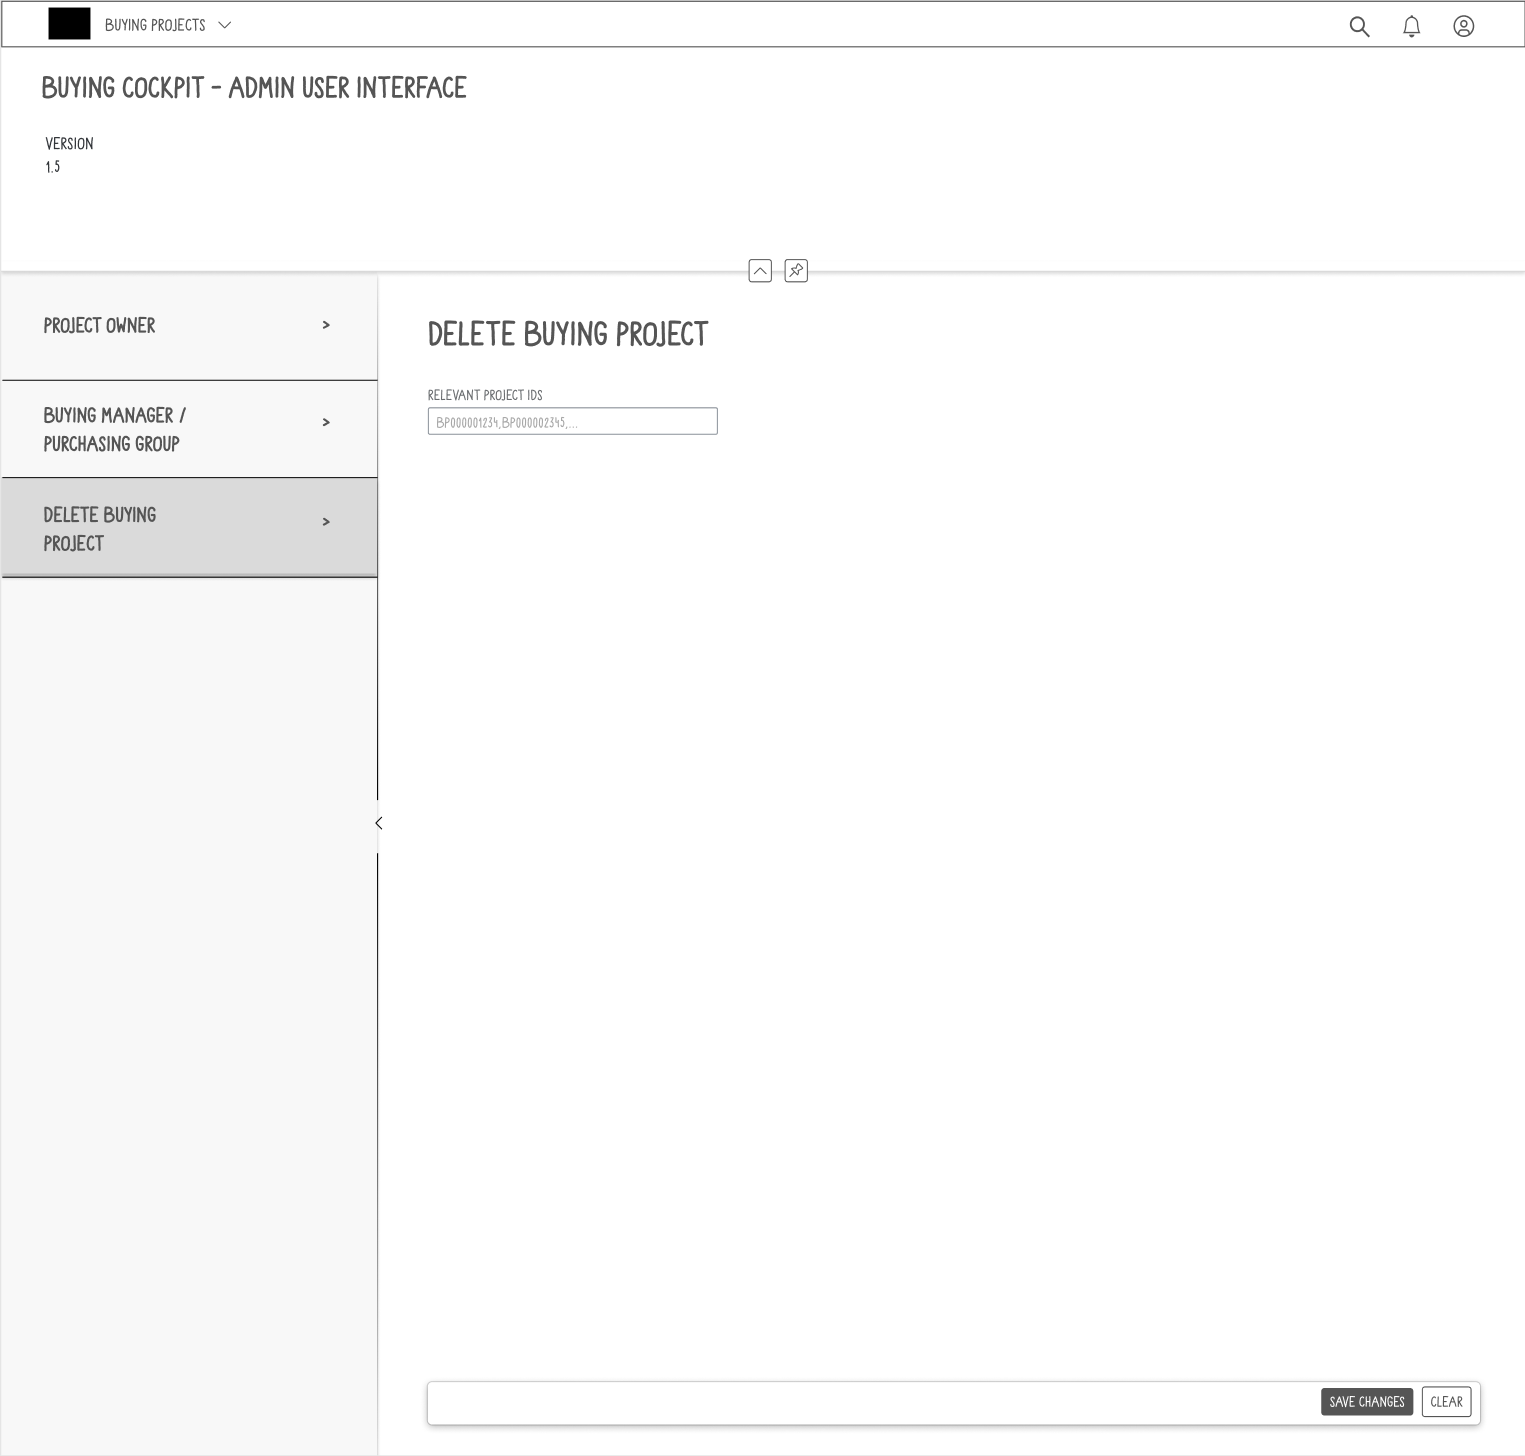
\includegraphics[width=\linewidth]{Images/Mockup_DEL_anonym.png}
    \caption[Mockup: Admin-UI Löschungs-Seite]{Mockup: Admin-UI Löschungs-Seite}
\end{figure}

\begin{figure}[H]
    \centering
    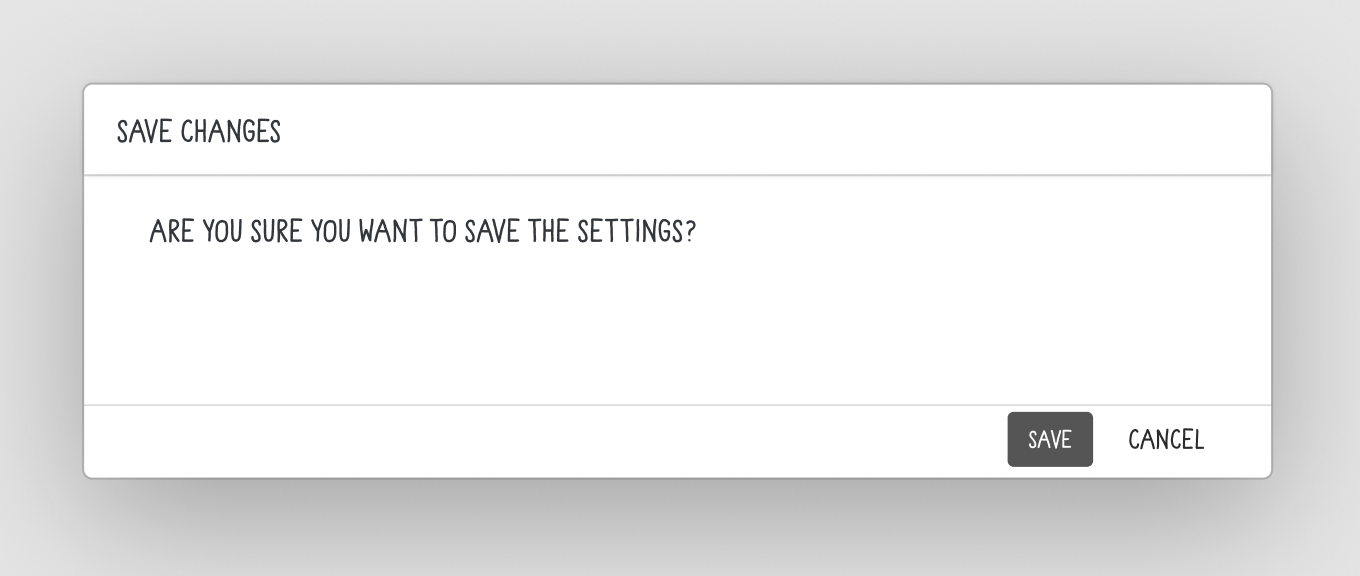
\includegraphics[width=\linewidth]{Images/Mockup_PopUp.png}
    \caption[Mockup: Admin-UI Pop-Up]{Mockup: Admin-UI Pop-Up}
\end{figure}

\subsection[Software-Design]{Software-Design}
Im folgenden Kapitel wird das Software-Design des Admin-UI und der dazu gehöhrenden Anwendung näher beschrieben.
Es bietet einen Überblick über die Architektur der Anwendung, die verwendeten Technologien und die Struktur der Daten.

\subsubsection[Grundlegende Architektur]{Grundlegende Architektur}
Die grundlegende Architektur der Anwendungen wird in Abbildung \ref{fig:architecture} etwas vereinfacht dargestellt, Komponenten, welche nicht relevant für die Entwicklung des Admin-UIs sind, wurden ausgelassen.

\begin{figure}[H]
    \centering
    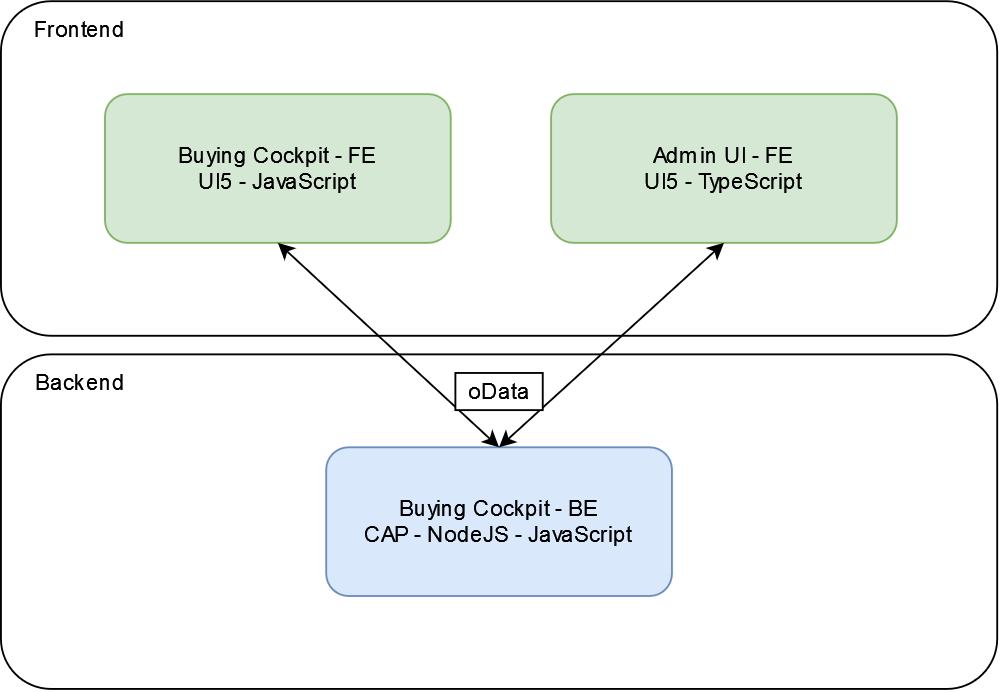
\includegraphics[width=\linewidth]{Images/BE_Architecture.png}
    \caption[Grundlegende Architektur der Anwendungen]{Grundlegende Architektur der Anwendungen}
    \label{fig:architecture}
\end{figure}
Die Architektur ist der Anwendungen ist in Frontend und Backend aufgeteilt und diese Ebenen kommunizieren über ein standartisiertes Protokol miteinander.

\begin{enumerate}
    \item \textbf{Frontend-Komponenten:}
    \begin{itemize}
        \item \textbf{Buying Cockpit - \gls{fe}:} \\
        Diese Komponente ist mit \gls{sapui5} und JavaScript entwickelt und bildet die Hauptanwendung und ist die Benutzeroberfläche für die Nutzer.
        \item \textbf{Admin-UI:} \\
        Dies ist die zu entwickelnde Administrationsoberfläche für das Buying Cockpit und  kann nur von bestimmten Nutzern verwendet werden.
    \end{itemize} 
    \item \textbf{Backend-Komponente:}
    \begin{itemize}
        \item \textbf{Buying Cockpit - \gls{be}:}
        Das Backend des Systems basiert auf \gls{cap} und wird mit NodeJS und JavaScript entwickelt.
        Es stellt die benötigten Daten und Services über standardisierte Schnittstellen beiden Frontend-Anwendungen zur Verfügung.
    \end{itemize}
    \item \textbf{Kommunikationsprotokoll:} \\
    Die Kommunikation zwischen dem Frontend und dem Backend erfolgt über das \textbf{OData-Protokol}. 
    \gls{odata} ermöglicht den standardisierten Austausch von Daten über HTTP und bietet eine effiziente Möglichkeit, auf Daten zuzugreifen und diese zu manipulieren.
\end{enumerate}
\subsubsection[Datenstruktur]{Datenstruktur}
Im folgenden wird die Datenstruktur für die Anwendungen vereinfacht dargestellt und Attribute, Entitäten und Relationen, welche nicht relevant für das Admin-UI sind, ausgelassen.

In Abbildung \ref{fig:datastructure} sind die drei Entitäten, welche im Admin-UI manipuliert werden sollen, in einen \gls{erm} dargestellt: \\
\begin{figure}[H]
    \centering
    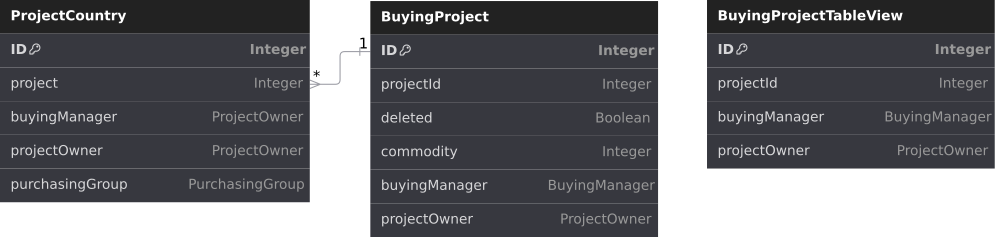
\includegraphics[width=\linewidth]{Images/Datenstruktur.png}
    \caption[Vereinfachte Darstellung der Datenstruktur]{Vereinfachte Darstellung der Datenstruktur}
    \label{fig:datastructure}
\end{figure}

Die Entität \textit{BuyingProjectTableView} ist eine Entität, welche für das Filtern auf der Übersichtsseite der BuyingCockpit Anwendung benötigt wird.
Daher müssen die Werte aus der \textit{BuyingProject}-Entität mit dieser übereinstimmen und somit immer beide simultan aktualisiert werden.